\let\lesson\undefined
\newcommand{\lesson}{\phantomlesson{Bài 20.}}
\setcounter{section}{2}
\section{Trắc nghiệm nhiều phương án lựa chọn}
\setcounter{ex}{0}
\Opensolutionfile{ans}[ans/VN10-Y24-PH-SYL-031P-TN]
% ===================================================================
\begin{ex}\mkstar{1}
	Biểu thức nào sau đây thể hiện mối liên hệ giữa tốc độ dài, tốc độ góc và chu kì quay?
	\choice
	{$v=\omega R=2\pi TR$}
	{$v=\dfrac{\omega}{R}=\dfrac{2\pi}{T}R$}
	{\True $v=\omega R=\dfrac{2\pi}{T}R$}
	{$v=\dfrac{\omega}{R}=\dfrac{2\pi}{TR}$}
	\loigiai{}
\end{ex}
% ===================================================================
\begin{ex}\mkstar{2}
Chuyển động của vật nào dưới đây được coi là chuyển động tròn đều?	
	\choice
	{Chuyển động của bánh xe ô tô khi đang hãm phanh}
	{\True Chuyển động của kim phút trên mặt đồng hồ chạy đúng giờ}
	{Chuyển động quay của các điểm treo các ghế ngồi trên chiếc đu quay}
	{Chuyển động quay của cánh quạt khi vừa tắt điện}
	\loigiai{Chuyển động của kim phút trên mặt đồng hồ chạy đúng giờ là chuyển động tròn đều.}
\end{ex}
% ===================================================================
\begin{ex}\mkstar{2}
	Các công thức liên hệ giữa tốc độ góc $\omega$ với chu kỳ $T$ và giữa tốc độ góc $\omega$ với tần số $f$ trong chuyển động tròn đều là gì?
	\choice
	{$\omega=2\pi T$; $\omega=\dfrac{2\pi}{f}$}
	{\True $\omega=\dfrac{2\pi}{T}$; $\omega=2\pi f$}
	{$\omega=2\pi T$; $\omega=2\pi f$}
	{$\omega=\dfrac{2\pi}{T}$; $\omega=\dfrac{2\pi}{f}$}
	\loigiai{Công thức liên hệ giữa tốc độ góc $\omega$ với chu kỳ $T$ là $\omega=\dfrac{2\pi}{T}$.
		Công thức liên hệ giữa giữa tốc độ góc $\omega$ với tần số $f$ trong chuyển động tròn đều là $\omega=2\pi f$.}
\end{ex}
% ===================================================================
\begin{ex}\mkstar{2}
Một bánh xe có đường kính $\SI{100}{\centi\meter}$ lăn đều với vận tốc $\SI{36}{\kilo\meter/\hour}$. Gia tốc hướng tâm của một điểm trên vành bánh xe có độ lớn	
	\choice
	{$\SI{200}{\meter/\second^2}$}
	{$\SI{400}{\meter/\second^2}$}
	{\True $\SI{100}{\meter/\second^2}$}
	{$\SI{300}{\meter/\second^2}$}
	\loigiai{Đổi đơn vị: $\SI{100}{\centi\meter}=\SI{1}{\meter}$; $\SI{36}{\kilo\meter/\hour}=\SI{10}{\meter/\second}$\\		
		Gia tốc hướng tâm của một điểm trên vành bánh xe có độ lớn:
		$$a_\text{ht}=\dfrac{v^2}{R}=\SI{100}{\meter/\second^2}.$$}
\end{ex}
% ===================================================================
\begin{ex}\mkstar{2}
	Một đĩa tròn bán kính $\SI{20}{\centi\meter}$ quay đều quanh trục của nó. Đĩa quay hết 1 vòng mất $\SI{0.2}{\second}$. Tốc độ dài $v$ của một điểm nằm ở mép đĩa bằng
	\choice
	{$\SI{4,71}{\meter/\second}$}
	{$\SI{3,14}{\meter/\second}$}
	{\True $\SI{6,28}{\meter/\second}$}
	{$\SI{7,85}{\meter/\second}$}
	\loigiai{Tốc độ dài $v$ của một điểm trên vành ngoài xe:
		$v=r\omega=r\dfrac{\Delta \alpha}{\Delta t}=\SI{0,2}{\meter}\dfrac{2\pi}{\SI{0.2}{\second}}=\SI{6,28}{\meter/\second}$}
\end{ex}
% ===================================================================
\begin{ex}\mkstar{2}
	Một động cơ xe máy có trục quay 1200 vòng/phút. Tốc độ góc của chuyển động quay là bao nhiêu?	
	\choice
	{\True $\SI{125,7}{\radian/\second}$}
	{$\SI{188,5}{\radian/\second}$}
	{$\SI{62,8}{\radian/\second}$}
	{$\SI{7200}{\radian/\second}$}
	\loigiai{Tốc độ góc của chuyển động quay là:
		$\omega$ = 1200 vòng/ phút = $1200\cdot\dfrac{2\pi}{60}\,\SI{}{\radian/\second}=\SI{125,7}{\radian/\second}$}
\end{ex}
% ===================================================================
\begin{ex}\mkstar{2}
Một bánh xe có bán kính $\SI{100}{\centi\meter}$ lăn đều với vận tốc $\SI{54}{\kilo\meter/\hour}$. Gia tốc hướng tâm của một điểm trên vành bánh xe có độ lớn	
	\choice
	{\True $\SI{225}{\meter/\second^2}$}
	{$\SI{400}{\meter/\second^2}$}
	{$\SI{100}{\meter/\second^2}$}
	{$\SI{300}{\meter/\second^2}$}
	\loigiai{Gia tốc hướng tâm của một điểm trên vành bánh xe có độ lớn:
		$$a_\text{ht}=\dfrac{v^2}{R}=\SI{225}{\meter/\second^2}.$$}
\end{ex}
% ===================================================================
\begin{ex}\mkstar{2}
	Xe đạp của một vận động viên chuyển động thẳng đều với $v=\SI{36}{km/h}$. Biết bán kính của lốp xe đạp là $\SI{32.5}{cm}$. Tính tốc độ góc và gia tốc hướng tâm tại một điểm trên lốp bánh xe.
	\choice
	{\True $\omega = \SI{30.77}{rad/s}$, $a_\text{ht} = \SI{307.7}{m/s^2}$}
	{$\omega = \SI{30.77}{rad/s}$, $a_\text{ht} = \SI{377.7}{m/s^2}$}
	{$\omega = \SI{3.77}{rad/s}$, $a_\text{ht} = \SI{30.7}{m/s^2}$}
	{$\omega = \SI{3.77}{rad/s}$, $a_\text{ht} = \SI{307.7}{m/s^2}$}
	\loigiai{Vận tốc xe đạp cũng là tốc độ dài của một điểm trên lốp xe:
		$$v=\SI{36}{km/h} = \SI{10}{m/s}$$
		Tốc độ góc:
		$$\omega = \dfrac{v}{R} = \SI{30.77}{rad/s}$$
		Gia tốc hướng tâm:
		$$a_\text{ht} = \dfrac{v^2}{R} = \SI{307.7}{m/s^2}$$}
\end{ex}
% ===================================================================
\begin{ex}\mkstar{2}
	Hai vật A và B chuyển động tròn đều với cùng chu kì trên hai đường tròn có bán kính khác nhau lần lượt là $R_\text A$ và $R_\text B$, với $R_\text A = 4 R_\text B$. Nếu vật A chuyển động với tốc độ dài $\SI{12}{m/s}$ thì tốc độ dài của vật B là
	\choice
	{$\SI{48}{m/s}$}
	{$\SI{24}{m/s}$}
	{\True $\SI{3}{m/s}$}
	{$\SI{4}{m/s}$}
	\loigiai{Vì $T_A=T_B\Rightarrow\omega_A=\omega_B
		$.\\		
		Lập tỉ lệ:
		$$\dfrac{v_\text A}{v_\text B} = \dfrac{R_\text A}{R_\text B} = 4 \Rightarrow v_\text B =\SI{3}{m/s} $$}
\end{ex}
% ===================================================================
\begin{ex}\mkstar{2}
	Hai vật A và B chuyển động tròn đều trên hai đường tròn tiếp xúc nhau. Chu kì của A là 4 s, còn chu kì của B là 2 s. Biết rằng tại thời điểm ban đầu chúng xuất phát cùng một lúc từ điểm tiếp xúc của hai đường tròn và chuyển động ngược chiều nhau. Khoảng thời gian ngắn nhất để hai vật gặp nhau lần nữa là
	\choice
	{$\SI{1}{\second}$}
	{$\SI{2}{\second}$}
	{\True $\SI{4}{\second}$}
	{$\SI{6}{\second}$}
	\loigiai{$T_A=2T_B$, để 2 vật gặp nhau thì vật A phải quay hết $k$ vòng với $k\in\mathbb{Z}$.\\
		Vậy khoảng thời gian ngắn nhất khi $k=1$, khi đó $$\Delta t= T_A=\SI{4}{\second}$$}
\end{ex}
	
\Closesolutionfile{ans}
\section{Trắc nghiệm đúng/sai}
\setcounter{ex}{0}
\Opensolutionfile{ans}[ans/VN10-Y24-PH-SYL-031P-TF]
% ===================================================================
\begin{ex}\mkstar{2}
Góc tạo bởi kim giờ và kim phút của một đồng hồ như hình bên.
\begin{center}
	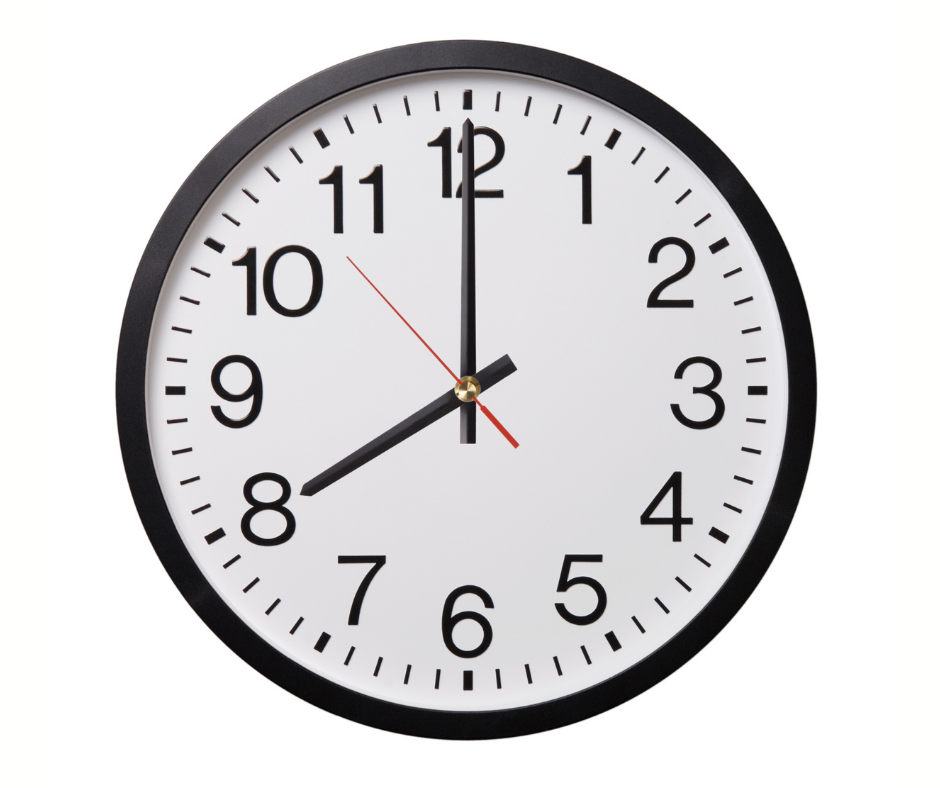
\includegraphics[scale=0.15]{../figs/VN10-Y24-PH-SYL-031P-1}
\end{center} 	
	\choiceTF[t]
	{Tại thời điểm trên hình, góc tạo bởi kim giờ và kim phút là $\SI{150}{\degree}$}
	{Sau 4 giờ, góc hợp bởi kim giờ và kim phút là $\SI{180}{\degree}$}
	{Kể từ thời điểm trên đến thời điểm 9 giờ, kim giờ đã quay được một góc bằng $\xsi{\dfrac{\pi}{3}}{\radian}$}
	{\True Khi kim phút quay được một vòng thì kim giờ quay được một góc $\xsi{\dfrac{\pi}{6}}{\radian}$}
	\loigiai{\begin{itemchoice}
			\itemch Sai. Góc tạo bởi kim giờ và kim phút là $\SI{120}{\degree}$.
			\itemch Sai. Sau đó 4 giờ, kim giờ trùng với kim phút.
			\itemch Sai. Đến thời điểm 9 giờ, kim giờ quay được một góc bằng $\xsi{\dfrac{\pi}{6}}{\radian}$.
			\itemch Đúng. Kim phút quay một vòng thì kim giờ quay được $\dfrac{1}{12}$ vòng nên góc quay được là $\xsi{\dfrac{\pi}{6}}{\radian}$.
	\end{itemchoice}}
\end{ex}
% ===================================================================
\begin{ex}\mkstar{2}
	Lồng giặt của một máy giặt TOSHIBA khi hoạt động ổn định thì có tốc độ quay từ $\SI{600}{\text{vòng/phút}}$ đến $\SI{1800}{\text{vòng/phút}}$ tùy thuộc vào chế độ giặt. Biết đường kính lồng giặt là $\SI{330}{\milli\meter}$.
	\choiceTF[t]
	{\True Tần số bé nhất của lồng giặt là $\SI{10}{\hertz}$}
	{Chu kì quay bé nhất của lồng giặt là $\SI{0.1}{\second}$}
	{Tốc độ chuyển động nhỏ nhất của một điểm trên thành lồng giặt khi máy đang chạy ổn định là $\SI{10.362}{\meter/\second}$}
	{Tốc độ chuyển động lớn nhất của một điểm trên thành lồng giặt khi máy đang chạy ổn định là $\SI{31.806}{\meter/\second}$}
	\loigiai{
	\begin{itemchoice}
		\itemch Đúng. $f_{\min}=\dfrac{600}{60}=\SI{10}{\hertz}$.
		\itemch Sai. $f_{\max}=\dfrac{1800}{60}=\SI{30}{\hertz}\Rightarrow T_{\min}=\xsi{\dfrac{1}{30}}{\second}$.
		\itemch Sai. $v_{\min}=\omega_{\min}R=2\pi f_{\min}R=\SI{20.735}{\meter/\second}$.
		\itemch Sai. $v_{\max}=\omega_{\max}R=2\pi f_{\max}R=\SI{62.2}{\meter/\second}$.
	\end{itemchoice}
	}
\end{ex}
\Closesolutionfile{ans}
\section{Tự luận}
\setcounter{ex}{0}
\Opensolutionfile{ans}[ans/VN10-Y24-PH-SYL-031P-TL]
% ======================================================================
\begin{ex}\mkstar{2}
	Một đầu cánh quạt quay với tần số 400 vòng/phút. Cánh quạt dài $\SI{0.8}{m}$. Tính tốc độ dài và tốc độ góc của một điểm ở đầu cánh quạt.
	\loigiai{Ta có tần số:
		$$f=400\ \text{vòng/phút} = \xsi{\dfrac{20}{3}}{\text{vòng/s}}$$
		Tốc độ góc của một điểm ở đầu cánh quạt:
		$$\omega = 2\pi f = \SI{41.89}{rad/s}$$
		Tốc độ dài:
		$$v=r \omega = \SI{33.5}{m/s}$$}
\end{ex}
% ======================================================================
\begin{ex}\mkstar{2}
	Một vệ tinh nhân tạo có quỹ đạo là một đường tròn cách mặt đất 400 km, quay quanh Trái Đất một vòng hết 90 phút. Gia tốc hướng tâm của vệ tinh là bao nhiêu? Cho bán kính Trái Đất $R=\SI{6389}{km}$.
	\loigiai{Ta có chu kì quay của vệ tinh là
		$$T=5400\ \text s$$
		Tốc độ góc:
		$$\omega = \dfrac{2\pi}{T} = \SI{1.16e-3}{rad/s}$$
		Gia tốc hướng tâm:
		$$a_\text{ht} =\left(R+h\right)\omega^2 \approx \SI{9.14}{m/s^2}$$}
\end{ex}
% ======================================================================
\begin{ex}\mkstar{2}
	Một đồng hồ treo tường có kim phút dài 10 cm và kim giờ dài 8 cm. Cho rằng các kim quay đều. Tính tốc độ dài và tốc độ góc của điểm đầu hai kim.
	\loigiai{	Bán kính kim phút: $R_\text p = \SI{0.1}{m}.$\\
		Chu kì quay của kim phút: $$T_\text p = 3600\ \text s$$
		Tốc độ góc của kim phút:
		$$\omega_\text p = \SI{1.74E-3}{\radian/\second}$$
		Tốc độ dài của kim phút:
		$$v_\text p = \SI{0.174}{\milli\meter/\second}$$
		Bán kính kim giờ: $R_\text g = \SI{0.08}{\meter}.$\\
		Chu kì quay của kim giờ: $$T_\text{g} = \SI{43200}{\second}$$
		Tốc độ góc của kim giờ:
		$$\omega_\text g = \SI{1.45E-4}{\radian/\second}$$
		Tốc độ dài của kim giờ:
		$$v_\text g = \SI{11.6E-3}{\milli\meter/\second}$$	}
\end{ex}
% ======================================================================
\begin{ex}\mkstar{2}
\immini{Một ròng rọc chuyển động tròn đều với tốc độ góc $\omega$, hai điểm A và B nằm trên cùng bán kính $R$ của một ròng rọc như hình vẽ.
	Điểm A nằm ngoài vành của ròng rọc có vận tốc $v_\text A = \SI{2.4}{m/s}$. Điểm B cách A $\SI{10}{cm}$ có vận tốc $v_\text B = \SI{0.8}{m/s}$. Coi ròng rọc chuyển động tròn đều quanh trục. Tính tốc độ góc $\omega$ và bán kính $R$ của ròng rọc.}
	{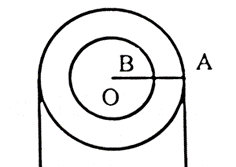
\includegraphics[scale=0.4]{../figs/VN10-2021-PH-TP006-1.png}}
	\loigiai{Hai điểm A và B có cùng tốc độ góc nên:
		$$\dfrac{R_\text{B}}{R_\text{A}} = \dfrac{v_\text{B}}{v_\text{A}}$$
		Với $R_\text{A} - R_\text{B} = \text{AB} = \SI{10}{cm}$, suy ra
		$$R_\text{A} =\SI{15}{cm}$$
		$$\omega=\SI{16}{rad/s}$$}
\end{ex}
		
% ======================================================================
\begin{ex}\mkstar{2}
	Xét một điểm nằm trên đường xích đạo trong chuyển động tự quay của Trái Đất. Biết bán kính Trái Đất tại xích đạo là $\SI{6400}{km}.$ Hãy tính chu kì chuyển động của điểm đó.
	\loigiai{Trái Đất quay một vòng 24h. Chu kỳ quay của một điểm nằm trên đường xích đạo quanh trục Trái Đất:
		$$T = \SI{24}{h} = \SI{86400}{s}.$$}
\end{ex}
% ======================================================================
\begin{ex}\mkstar{2}
	Xét một điểm nằm trên đường xích đạo trong chuyển động tự quay của Trái Đất. Biết bán kính Trái Đất tại xích đạo là $\SI{6400}{km}.$ Hãy tính tốc độ và tốc độ góc của điểm đó.
	\loigiai{Tốc độ góc của điểm đó là: 
		$$\omega = \dfrac{2\pi}{T} = \text{7,3} \cdot 10^{-5}\ \text{rad/s}.$$
Tốc độ của điểm đó là:
$$v = \omega r = \SI{467,2}{m/s}.$$}
\end{ex}
% ======================================================================
\begin{ex}\mkstar{2}
Một đồng hồ điểm 3h30ph. Hãy tính góc quay từ vị trí 12h đến vị trí của kim phút và kim giờ.	
	\loigiai{Kim phút: Tại 12h kim phút chỉ số 12, đến 3h30p thì kim phút chỉ số 6, ta thấy kim phút đi được một nửa vòng tròn.($180^\circ$)\\
Kim giờ: 1 giờ, kim giờ quay được 1 góc $30^\circ$.\\
Từ 12h đến 3h30p tương ứng là 3,5h thì kim giờ quay được 1 góc là 3,5$\cdot 30^\circ = 105^\circ.$}
\end{ex}
% ======================================================================
\begin{ex}\mkstar{2}
	Một em bé cưỡi ngựa gỗ trên sàn quay, ở cách trục quay $\SI{2,1}{m}$. Tốc độ góc của sàn quay là $\SI{0,42}{rad/s}$. Tính tốc độ của ngựa gỗ.	
	\loigiai{Tốc độ của ngựa:
		$$v = \omega r = \SI{0,882}{m/s}.$$}
\end{ex}
% ======================================================================
\begin{ex}\mkstar{2}
Tính gia tốc hướng tâm của Mặt Trăng trong chuyển động quay quanh Trái Đất (coi Mặt Trăng chuyển động tròn đều quanh Trái Đất). Biết khoảng cách từ Mặt Trăng đến tâm Trái Đất là $\text{3,84}\cdot 10^8\ \text{m}$ và chu kì quay là 27,2 ngày.	
	\loigiai{Đổi 27,2 ngày = $\SI{2 350 080}{s}.$\\
			Gia tốc hướng tâm của Mặt Trăng là:
			$$a = \omega^2 r = \text{2,74}\cdot 10^{-3}\ \text{m/s}^2.$$}
\end{ex}
% ======================================================================
\begin{ex}\mkstar{3}
Trạm không gian quốc tế ISS có tổng khối lượng 350 tấn, quay quanh Trái Đất ở độ cao $\SI{340}{km}$ nơi có gia tốc trọng trường $\SI{8,8}{m/s^2}$. Bán kính Trái Đất là $\SI{6400}{km}$. Xác định số vòng trạm không gian thực hiện quanh Trái Đất trong một ngày.	
	\loigiai{Tốc độ góc trong chuyển động quay của trạm ISS quanh Trái Đất:
		$$a_\text{ht}=g=\omega^2\left(R+h\right)\Rightarrow \omega=\sqrt{\dfrac{g}{R+h}}=\sqrt{\dfrac{\SI{8.8}{\meter/\second^2}}{\SI{6400E3}{\meter}+\SI{340E3}{\meter}}}\approx\SI{1.14E-3}{\radian/\second}$$
		Số vòng trạm không gian thực hiện quanh Trái Đất trong một ngày
		$$n = \dfrac{t}{T} = \dfrac{t}{\dfrac{2\pi}{\omega}}\approx\SI{15.7}{\text{vòng}}.$$
		}
\end{ex}
% ======================================================================
\begin{ex}\mkstar{3}
Một trái bóng được buộc vào một sợi dây và quay tròn đều trong mặt phẳng ngang như hình \ref{fig:31-P-1}. Trái bóng quay một vòng trong $\SI{1}{\second}$ với tốc độ $\SI{0.5}{\meter/\second}$. Tính bán kính quỹ đạo và chiều dài $L$ của sợi dây, biết góc hợp bởi dây và phương thẳng đứng bằng $\SI{30}{\degree}$.
\begin{center}
	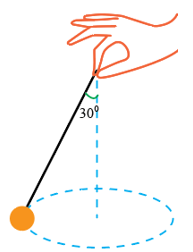
\includegraphics[width=0.2\linewidth]{../figs/VN10-2023-PH-TP031-P-1}
	\captionof{figure}{}
	\label{fig:31-P-1}
\end{center}	
	\loigiai{Chu kì quay của bóng: $T=\SI{1}{\second}$.\\
		Tốc độ góc của bóng:
		$$\omega=\dfrac{2\pi}{T}=\xsi{2\pi}{\radian/\second}$$
		Bán kính quỹ đạo của bóng:
		$$R=\dfrac{v}{\omega}=\dfrac{\SI{0.5}{\meter/\second}}{\xsi{2\pi}{\radian/\second}}\approx\SI{0.08}{\meter}.$$
		Chiều dài dây treo:
		$$L=\dfrac{R}{\sin\SI{30}{\degree}}=\SI{0.16}{\meter}.$$}
\end{ex}
% ======================================================================
\begin{ex}\mkstar{3}
	Coi Trái Đất là hình cầu có bán kính $R=\SI{6400}{\kilo\meter}$ và quay quanh trục với chu kì $\SI{24}{\hour}$. Tính gia tốc hướng tâm do Trái Đất chuyển động quanh trục gây ra cho một người đang đứng ở xích đạo và một người đứng ở vĩ tuyến $\SI{60}{\degree}$.
	\loigiai{Tốc độ góc trong chuyển động tự quay quanh trục của Trái Đất:
		$$\omega=\dfrac{2\pi}{T}=\dfrac{2\pi}{24\cdot\SI{3600}{\second}}=\xsi{\dfrac{\pi}{43200}}{\radian/\second}$$
		Gia tốc hướng tâm của người đứng ở xích đạo:
		$$a_1=\omega^2 R=\left(\xsi{\dfrac{\pi}{43200}}{\radian/\second}\right)^2\cdot\left(\SI{6400E3}{\meter}\right)\approx\SI{0.034}{\meter/\second^2}$$
		Gia tốc hướng tâm của người đứng ở vĩ tuyến $\SI{60}{\degree}$:
		$$a_2=\omega^2 R\cos\SI{60}{\degree}=\left(\xsi{\dfrac{\pi}{43200}}{\radian/\second}\right)^2\cdot\left(\SI{6400E3}{\meter}\right)\cdot\cos\SI{60}{\degree}\approx\SI{0.017}{\meter/\second^2}.$$}
\end{ex}
\Closesolutionfile{ans}